\documentclass[border=2pt]{standalone}
\usepackage{pgfplots}
\usepgfplotslibrary{fillbetween}
\usetikzlibrary{patterns}
\pgfplotsset{compat=1.18}
\definecolor{paper}{HTML}{FFFFFF}
\definecolor{tile}{HTML}{F3F4F6}
\definecolor{rule}{HTML}{C9CDD3}
\definecolor{ink}{HTML}{1B1D21}
\definecolor{muted}{HTML}{5D636B}
\definecolor{accent}{HTML}{1F5FD1}
\definecolor{red}{HTML}{C62828}
\definecolor{green}{HTML}{2E7D32}
\definecolor{orange}{HTML}{D7600A}
\definecolor{blue}{HTML}{1565C0}
\pagecolor{tile}
\color{ink}
\pgfplotsset{every axis/.append style={axis line style={muted}, tick style={muted}, tick label style={ink, font=\tiny},
  label style={ink, font=\tiny}, title style={ink, font=\tiny}, legend style={fill=tile, draw=rule, text=ink, font=\tiny}},
  every colorbar/.append style={tick label style={font=\tiny}}}
\begin{document}

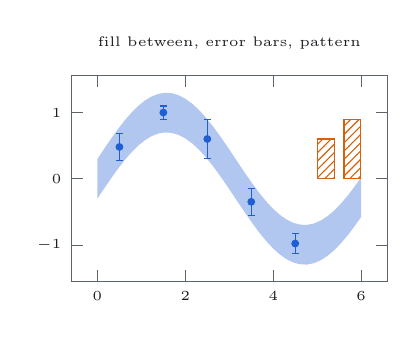
\begin{tikzpicture}
\begin{axis}[width=5.6cm, height=4.2cm, title={fill between, error bars, pattern}, cycle list={{accent},{red},{green}}]
\addplot[name path=a, draw=none, domain=0:6, samples=40] {sin(deg(x))+0.3};
\addplot[name path=b, draw=none, domain=0:6, samples=40] {sin(deg(x))-0.3};
\addplot[accent, fill opacity=0.35] fill between[of=a and b];
\addplot+[only marks, mark size=1.2pt, error bars/.cd, y dir=both, y explicit] coordinates
  {(0.5,0.48) +- (0,0.2) (1.5,1.0) +- (0,0.1) (2.5,0.6) +- (0,0.3) (3.5,-0.35) +- (0,0.2) (4.5,-0.98) +- (0,0.15)};
\addplot[ybar, bar width=6pt, pattern=north east lines, pattern color=orange, draw=orange] coordinates {(5.2,0.6) (5.8,0.9)};
\end{axis}
\end{tikzpicture}
\end{document}
